% Lecture Template for ME3023 -  Measurements in Mechanical Systems - Tennessee Technological University
% Spring 2020 - Summer 2020 - Fall 2020 - Spring 2021 - Summer 2021 - Fall 2023
% Tristan Hill, May 07, 2020 - June 12, 2020 - July 08, 2020 - Novemeber 02, 2020 - March 28, 2021 - May 25, 2021 - August 21, 2022 - September 02, 2023 - September 09, 2023 

% Fall 2023 - condensing and streamlining lectures by combining topics into a single PDF under the module name
%			  this will simplify file and link management as well as make lectures easier to use in class
%			- added image/ to clean directory and reduce redundancy, specific to module for now  

% updated Fall 2025

% Module Name: - Probability and Statistics
% Topic 1 - 
% Topic 2 - 
% Topic 3 - 

\documentclass[fleqn]{beamer} % for presentation (has nav buttons at bottom)
\usepackage{../measurements_lectures}
\usepackage{listings}

\author{ME3023 - Measurements in Mechanical Systems} 

\newcommand{\MNUM}{4\hspace{2mm}} % module number 
\newcommand{\moduletitle}{Probability and Statistics}

\newcommand{\sectionItitle}{Histograms and Probability Density Functions}
\newcommand{\sectionIItitle}{Characterizing a Population of Data}
\newcommand{\sectionIIItitle}{Z Table Examples}

\newcommand{\sectionIsubsectionItitle}{A Population of Data}
\newcommand{\sectionIsubsectionIItitle}{Randomly Distributed Data}
\newcommand{\sectionIsubsectionIIItitle}{Frequency Histogram}
\newcommand{\sectionIsubsectionIVtitle}{Probability Density Function}

\newcommand{\sectionIIsubsectionItitle}{A Population of Data}
\newcommand{\sectionIIsubsectionIItitle}{Variance and Standard Deviation}
\newcommand{\sectionIIsubsectionIIItitle}{Using the Z Table}
\newcommand{\sectionIIsubsectionIVtitle}{Example: Using the Z Table}

\newcommand{\sectionIIIsubsectionItitle}{Table of Probability Values}
\newcommand{\sectionIIIsubsectionIItitle}{Example 1}
\newcommand{\sectionIIIsubsectionIIItitle}{Example 2}
\newcommand{\sectionIIIsubsectionIVtitle}{Example 3}

 \newcommand{\btVFill}{\vskip0pt plus 1filll}

% custom box
\newsavebox{\mybox}

\title{Lecture Module - \moduletitle}

\date{Mechanical Engineering\vspc Tennessee Technological University}

\begin{document}

	\lstset{language=MATLAB,basicstyle=\ttfamily\small,showstringspaces=false}

	\frame{\titlepage \center\begin{framed}\Large \textbf{Module \MNUM - \moduletitle}\end{framed} \vspace{5mm}}

	% Module Outline
	\begin{frame} 
		\large \textbf{Module \MNUM - \moduletitle} \vspace{3mm}\\

		\begin{itemize}
			\item Topic 1 - \hyperlink{sectionI}{\sectionItitle} \vspc % section I
			\item Topic 2 - \hyperlink{sectionII}{\sectionIItitle} \vspc % section II
			\item Topic 3 - \hyperlink{sectionIII}{\sectionIIItitle} \vspc % section III
		\end{itemize}

	\end{frame}

	% section I
	\section{\sectionItitle}\label{sectionI}

		% section I Outline
		\begin{frame} 
			\large \textbf{Topic 1 - \sectionItitle} \vspace{3mm}\\

			\begin{itemize}
				\item \hyperlink{sectionIsubsectionI}{\sectionIsubsectionItitle} \vspc %  section I subsection I
				\item \hyperlink{sectionIsubsectionII}{\sectionIsubsectionIItitle} \vspc % section I subsection II
				\item \hyperlink{sectionIsubsectionIII}{\sectionIsubsectionIIItitle} \vspc % section I subsection III
				\item \hyperlink{sectionIsubsectionIV}{\sectionIsubsectionIVtitle} \vspc % section I subsection IV
			\end{itemize}
		\end{frame}
		
		% section I subsection I 
		\subsection{\sectionIsubsectionItitle}\label{sectionIsubsectionI}

			\begin{frame}
				\frametitle{\sectionIsubsectionItitle}

				Consider a manufacturer that makes 100000 of ball bearings in a set. \vspace{3mm}

				\includegraphics[scale=.1]{images/bearing_fig1.jpg} \hspace{10mm}
				\includegraphics[scale=.1]{images/bearing_fig2.png} \hspace{10mm}
				\includegraphics[scale=.1]{images/bearing_fig3.jpeg}
				\begin{itemize}		
					\item How does the manufacturer ensure the quality of the product?
					\item How the does the seller communicate this to the buyer?
					\item How does the engineer use this information? 
				\end{itemize}

				{\tiny Images: \href{https://en.wikipedia.org/wiki/Ball_bearing}{Wikipedia} }
							

			\end{frame}

			\begin{frame}
				\frametitle{\sectionIsubsectionItitle}
				\bigskip

				The data set, or population, is generated by taking measurements of individuals chosen randomly from the entire population. \\ 
		 
				 {\bf \RD Sampling} refers to repeated measurements of the {\bf \PR measured variable} under fixed operating condition.	\\
				 
				 \[ X = \{ x_1,x_2,x_3, ... , x_i , ... , x_{n-1}, x_{n} \}  \]

			\end{frame}

		% section I subsection II
		\subsection{\sectionIsubsectionIItitle}\label{sectionIsubsectionII}

			\begin{frame}
				\frametitle{\sectionIsubsectionIItitle}

				Our discussion will assume that the values in the data set are {\bf \PN randomly distributed } about a mean value. It is important to consider what this means.
				
			\end{frame}

		% section I subsection III
		\subsection{\sectionIsubsectionIIItitle}\label{sectionIsubsectionIII}
			\begin{frame} 
				\frametitle{\sectionIsubsectionIIItitle}
				\bigskip

					"A {\GR histogram} is an accurate representation of the distribution of numer-
					ical data. It is an estimate of the probability distribution of a continuous
					variable (CORAL ) and was first introduced by Karl Pearson.[1] It differs
					from a bar graph, in the sense that a bar graph relates two variables, but a
					histogram relates only one." - Wikipedia

			\end{frame}	

			\begin{frame}[containsverbatim] 
				\frametitle{\sectionIsubsectionIIItitle}

				Consider sampling the 0.5 inch diameter ball bearings with $\sigma=.001$.

				\lstset{basicstyle=\scriptsize}

				\begin{lstlisting}
0.5016 0.4991 0.4981 0.5003 0.4988 0.5007 0.4994 0.5000 0.4999 0.4999 0.4988  
0.4997 0.4991 0.4986 0.5000 0.5018 0.4996 0.5010 0.4991 0.5011 0.5006 0.5006  
0.5014 0.5001 0.4997 0.4994 0.5001 0.5009 0.5009 0.4992 0.4983 0.5004 0.5005 
0.5004 0.4992 0.5009 0.5003 0.5018 0.5004 0.4996 0.5014 0.4992 0.4986 0.5002 
0.4986 0.4992 0.5003 0.5002 0.4999 0.4998 0.5013 0.5009 0.5003 0.4986 0.4991
0.5030 0.4995 0.5012 0.5005 0.4992 0.4995 0.5005 0.5000 0.5005 0.4993 0.4987 
0.4992 0.5018 0.4976 0.5003 0.4991 0.5007 0.5002 0.4980 0.5004 0.5000 0.4997 
0.5002 0.5004 0.4980 0.5011 0.5003 0.5013 0.5000 0.5001 0.5003 0.5000 0.5013  
0.5004 0.4988 0.5003 0.4999 0.5004 0.4996 0.4999 0.5000 0.4993 0.5003 0.4996  
0.4992 0.5008 0.4997 0.5004 0.4998 0.4998 0.5006 0.5002 0.5010 0.5014 0.5019
0.5008 0.4997 0.5002 0.4993 0.4995 0.5007 0.4986 0.5009 0.4999 0.5002 0.5010  
0.4996 0.4993 0.4982 0.4994 0.4993 0.4995 0.5002 0.5004 0.4999 0.5005 0.4993 
				\end{lstlisting}

				{\tiny Data: Generated in MATLAB, see probabilty\_statistics\_topic1.m }
				
			\end{frame}	

			\begin{frame} 
				\frametitle{\sectionIsubsectionIIItitle}
				\bigskip
				\scriptsize Draw Historgram by hand 
				\includegraphics[scale=.20]{images/graph_paper_80_30.png}		


			\end{frame}

			\begin{frame} 
				\frametitle{\sectionIsubsectionIIItitle}
				\bigskip

	

			\end{frame}



		% section I subsection IV
		\subsection{\sectionIsubsectionIVtitle}\label{sectionIsubsectionIV}	

			\begin{frame} \scriptsize
				\frametitle{\sectionIsubsectionIVtitle}

				\bigskip
\textbf{Activity:} Complete as an individual, discussion with peers is encouraged.\\
      Write a MATLAB progam to do the following:
			\begin{enumerate}
		    \item Generate a population of data that is randomly distributed about a central mean to represent a repeated measurement or physical property. One suggestion is to use the built-in function {\it normrnd() }. Choose the population size, mean value, and standard deviation.
        \item Show the data in a labeled figure with item number on the x-axis and measured value on the y-axis.  
    %		\item Sample 20 values from the population on the previous slide. It will help to write them down in a collumn. 
				\item Create a histogram using the population of data. One option is to use the MATLAB function {\it histogram()}. Choose an appropriate bin size for the histogram to represent the data. The goal is to show the central tendancy and random distribution of the population of data.
		    \item Show a continuous probability density function to represent the data. The function should have the same mean value and standard deviation as used above.
      	\end{enumerate}

		\textbf{Deliverables:} Upload your MATLAB code to the appropriate folder as a .m file {\it Concept Example: Sketch Histograms and Probabilty Density Functions}. Include your name, date, and topic in the program file.	

				
			\end{frame}

			\begin{frame}
				\frametitle{\sectionIsubsectionIVtitle}

\bigskip


			\end{frame}

	
	% Section II
	\section{\sectionIItitle}\label{sectionII}

		% section II Outline
		\begin{frame}
			\large \textbf{Topic 2 - \sectionIItitle} \vspace{3mm}\\

			\begin{itemize}
				\item \hyperlink{sectionIIsubsectionI}{\sectionIIsubsectionItitle} \vspc %  section II subsection I
				\item \hyperlink{sectionIIsubsectionII}{\sectionIIsubsectionIItitle} \vspc % section II subsection II
				\item \hyperlink{sectionIIsubsectionIII}{\sectionIIsubsectionIIItitle} \vspc % section II subsection III
				\item \hyperlink{sectionIIsubsectionIV}{\sectionIIsubsectionIVtitle} \vspc % section II subsection IV
			\end{itemize}

		\end{frame}

		% section II subsection I
		\subsection{\sectionIIsubsectionItitle}\label{sectionIIsubsectionI}

			\begin{frame}[label=sectionIIsubsectionI]
				\frametitle{\sectionIIsubsectionItitle}

        Review from topic 1:\vspace{2mm}\\
				
        Consider a manufacturing facility that makes ball bearings. 
				\begin{itemize}		
					\item How does the manufacturer ensure the quality of the product?
					\item How the does the seller communicate this to the buyer?
					\item How does the Engineer use this information? 
				\end{itemize}

			\end{frame}

			\begin{frame}[label=sectionIIsubsectionI]
				\frametitle{\sectionIIsubsectionItitle}
        Review from topic 1:\vspace{2mm}\\
				
The data set, or population, is generated by taking measurements of individuals chosen randomly from the entire population. \\ 
		 
				 {\bf \RD Sampling} refers to repeated measurements of the {\bf \PR measured variable} under fixed operating condition.	\\
				 
				 \[ X = \{ x_1,x_2,x_3, ... , x_i , ... , x_{n-1}, x_{n} \}  \]
			\end{frame}
		
			\begin{frame}[label=sectionIIsubsectionI]
				\frametitle{\sectionIIsubsectionItitle}
			 
        \textbf {Consider the dataset as a population of data or a {\it distribution}}.\vspace{2mm}\\  
 
        \begin{itemize}
          \item  What does the distribution look like?
          \item  How can we describe it mathematically? 
          \item  What function p(x) appropriately describes the distribution?  
        \end{itemize}

\vspace{3mm} 
\begin{multicols}{4}      
  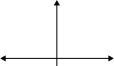
\includegraphics[scale=.225]{images/distribution_axes.png}     
  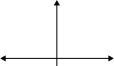
\includegraphics[scale=.225]{images/distribution_axes.png}     
  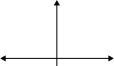
\includegraphics[scale=.225]{images/distribution_axes.png}     
  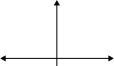
\includegraphics[scale=.225]{images/distribution_axes.png}     
\end{multicols}

      \end{frame}
      
		
			\begin{frame}[label=sectionIIsubsectionI]
				\frametitle{\sectionIIsubsectionItitle}\scriptsize
			 
        \textbf {It has been proposed that physical systems behave randomly}.\vspace{2mm}\\ 
        \begin{itemize}
          \item population of data shows central tendancy about a mean value
          \item the distribution can be described by the Gaussian, or normal distribution
          \item the assumption of the distribution model can be used to make predictions about population
        \end{itemize} 
 \begin{multicols}{2}
  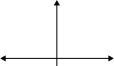
\includegraphics[scale=.5]{images/distribution_axes.png}     
  \[p(x)=\frac{1}{\sigma\left(2\pi\right)^{\left(1/2\right)}}exp\left[-\frac{1}{2}\frac{\left(x-x'\right)^2}{\sigma^2}\right] \]        
  \end{multicols}
    \end{frame}
      
      \begin{frame}[label=sectionIIsubsectionI]
				\frametitle{\sectionIIsubsectionItitle}

				\textbf{For a given set of measurements  we want to quantify:}
				\begin{itemize}
          
					\item a representative value that characterizes the average of the measured data set
					\item a representative value that provides a measure of the variation in the data set
					\item how well the average of the measured data set represents the average of the entire population
				\end{itemize}

			\end{frame}	

		% section II subsection II
		\subsection{\sectionIIsubsectionIItitle}\label{sectionIIsubsectionII}

			\begin{frame}
				\frametitle{\sectionIIsubsectionIItitle}
        Remember the histogram gernerated previously
        \[ N=\Sigma_{j=1}^Kn_j \]
      
        If you convert the value at each bin to a percentage, the area under the curve equals 100\%.

        \[100x\Sigma_{j=1}^Kf_i=100\% \]

			\end{frame}

			\begin{frame}
				\frametitle{\sectionIIsubsectionIItitle}
        
        Given the assumption that the variation in data is free from systematic errors, we can quantify the population with the following terms

      \[ x' = lim_{T\rightarrow\infty}\frac{1}{T}\int_0^Tx(t)dt  \]
      \[ x' = \int_{-\infty}^\infty xp(x)dx \]
      
       For discrete data this becomes
\[x'= lim_{T\rightarrow\infty}\frac{1}{N}\Sigma_{i=1}^N x_i \]

			\end{frame}
			
      \begin{frame}
				\frametitle{\sectionIIsubsectionIItitle}

				\begin{multicols}{2} \scriptsize
				The true variance is:\\
				\[ \sigma^2=\int\limits_{-\infty}^{\infty}(x-x')^2p(x)dx \]
				For discrete data this becomes:\\
				\[ \sigma^2=\lim\limits_{N\rightarrow \infty}\frac{1}{N}\sum\limits_{i=1}^{N}(x_i-x')^2 \]
				The square root of the {\bf \BL variance} \\
				is the {\bf \PR standard deviation}. \\
				\[\sigma=\sqrt{\sigma^2}\]

				\hspace*{-1.5cm}\includegraphics[scale=.20]{images/topic2_measured_fig2.png}		
				
				\end{multicols}

			\end{frame}

			\begin{frame}
				\includegraphics[scale=.50]{images/lecture1_fig1.png}
			\end{frame}

			\begin{frame}
				\includegraphics[scale=.50]{images/lecture1_fig1.png}
			\end{frame}

		% section II subsection III
		\subsection{\sectionIIsubsectionIIItitle}\label{sectionIIsubsectionIII}

			\begin{frame}
				\frametitle{\sectionIIsubsectionIIItitle}

				... The area under the portion of the probability density function curve, $p(x)$, defined by the interval $x'-z_1\sigma \leq x \leq x' +z_1\sigma$ provides the probability that a measurement will assume a value within that interval. Direct integration of $p(x)$ for a normal
				distribution between the limits $x'\pm z_1\sigma$ yields that for $z_1=1, 68.26\%$ of the area under $p(x)$ lies
				within $\pm 1\sigma$   $x'$ . This means that there is a $68.26\%$ chance that a measurement of $x$ will have a
				value within the interval $x'\pm 1\sigma$.
			
			\end{frame}		

			\begin{frame}
				\frametitle{\sectionIIsubsectionIIItitle}

				\bigskip


				\includegraphics[scale=.250]{images/topic2_fig4.png}
				
				$ z_1=1, 68.26\% $ of the area under $ p(x) $ lies within $ \pm z_1\sigma $ of $ x' $.\\ 
				$ z_1=2, 95.45\% $ of the area under $ p(x) $ lies within $ \pm z_1\sigma $ of $ x' $.\\ 
				$ z_1=3, 99.73\% $ of the area under $ p(x) $ lies within $ \pm z_1\sigma $ of $ x' $.\\ 		


			\end{frame}

			\begin{frame}
				\frametitle{\sectionIIsubsectionIIItitle}
						It follows directly that the representative value that characterizes a measure of the variation in a
				measured data set is the standard deviation. The probability that the ith measured value of x will
				have a value between $x' \pm z_1 \delta$ is $2 \times P(z_1) \times 100 = P\%$. \\

					This is written as \\
					
						\[ x_i = x' \pm z_1\sigma \hspace{3mm} (P\%) \]        
						
			

			\end{frame}

			\begin{frame}
			\frametitle{\sectionIIsubsectionIIItitle}





			\end{frame}

		% section II subsection IV 
		\subsection{\sectionIIsubsectionIVtitle}\label{sectionIIsubsectionIV}

			\begin{frame}
				\frametitle{\sectionIIsubsectionIVtitle}

		\includegraphics[scale=.25]{images/topic2_fig2.png}	
		\includegraphics[scale=.45]{images/topic2_fig3.png}


			\end{frame}

			\begin{frame}
				\frametitle{\sectionIIsubsectionIVtitle}



			\end{frame}

			\begin{frame}



			\end{frame}


		
	% Section III
	\section{\sectionIIItitle}\label{sectionIII}

		% section III Outline
		\begin{frame}
			\large \textbf{Topic 3 - \sectionIIItitle} \vspace{3mm}\\

			\begin{itemize}
				\item \hyperlink{sectionIIIsubsectionI}{\sectionIIIsubsectionItitle} \vspc %  section III subsection I
				\item \hyperlink{sectionIIIsubsectionII}{\sectionIIIsubsectionIItitle} \vspc % section III subsection II
				\item \hyperlink{sectionIIIsubsectionIII}{\sectionIIIsubsectionIIItitle} \vspc % section III subsection III
				\item \hyperlink{sectionIIIsubsectionIV}{\sectionIIIsubsectionIVtitle} \vspc % section III subsection IV
			\end{itemize}

		\end{frame}

		% section III subsection I
		\subsection{\sectionIIIsubsectionItitle}\label{sectionIIIsubsectionI}

			\begin{frame}
				\frametitle{\sectionIIIsubsectionItitle}

				\includegraphics[scale=.3]{images/topic2_fig2.png}	
				\includegraphics[scale=.3]{images/topic2_fig3.png}	
				
			\end{frame}

			\begin{frame}
				\frametitle{\sectionIIIsubsectionItitle}


		
			\end{frame}

		% section III subsection II
		\subsection{\sectionIIIsubsectionIItitle}\label{sectionIIIsubsectionII}	

			\begin{frame}
				\frametitle{\sectionIIIsubsectionIItitle}

						Using the probability values in Table 4.3, show that the probability that a measurement will yield a
value within $x'\pm \sigma$ is $0.6826$ or $68.26\%$.

		\vspace{30mm}
	

			\end{frame}

		% section III subsection III
		\subsection{\sectionIIIsubsectionIItitle}\label{sectionIIIsubsectionIII}

			\begin{frame}
				\frametitle{\sectionIIIsubsectionIIItitle}

		Now consider the measurements from the ball bearing factory in topic 1. 
		
		\includegraphics[scale=.2]{images/topic3_fig1.png}	
	
		
			
		
		\vspace{30mm}
		

			\end{frame}

			\begin{frame}
				\frametitle{\sectionIIIsubsectionIIItitle}



	If the true mean is 0.5 inches, what is the probability that a individual bearing will measure within 0.45 $\sigma$ of the mean ? What about 0.15 $\sigma$? \\
		\vspace{30mm}


			\end{frame}

			\begin{frame}

		What is the probability that a individual bearing will measure between 0.44 and 0.49 inches? 
			%\vspace{30mm}

			\end{frame}

			\begin{frame}

				If the true mean is 0.5 inches, estimate the uncertainty interval at a probability of 70\%. Also estimate the uncertainty interval at a probability of 90\%.
	What is the probability that a individual bearing will measure within 0.45 $\sigma$ of the mean ? What about 0.15 $\sigma$? \\
		%\vspace{30mm}


			\end{frame}

		% section III subsection IV
		\subsection{\sectionIIIsubsectionIVtitle}\label{sectionIIIsubsectionIV}	

			\begin{frame}
				\frametitle{\sectionIIIsubsectionIVtitle}

				What is the probability that a individual bearing will measure between 0.40 and 0.44 inches? What is different about this problem? What is the significance of the $z$ value not present in the table?		


			\end{frame}

			\begin{frame}
				\frametitle{\sectionIIIsubsectionIVtitle}
				


			\end{frame}

\end{document}





